% ----------------------------------------------------------------
% achemso --- Support for submissions to American Chemical
%  Society journals
% Maintained by Joseph Wright
% E-mail: joseph.wright@morningstar2.co.uk
% Originally developed by Mats Dahlgren
%  (c) 1996-98 by Mats Dahlgren
%  (c) 2007-2008 Joseph Wright
% Released under the LaTeX Project Public license v1.3c or later
% See http://www.latex-project.org/lppl.txt
%
% Part of this bundle is derived from cite.sty, to which the
% following license applies:
%   Copyright (C) 1989-2003 by Donald Arseneau
%   These macros may be freely transmitted, reproduced, or
%   modified provided that this notice is left intact.
% ----------------------------------------------------------------
%
% The achemso bundle provides a LaTeX class file and BibTeX style
% file in accordance with the requirements of the American
% Chemical Society.  The files can be used for any documents, but
% have been carefully designed and tested to be suitable for
% submission to ACS journals.
%
% The bundle also includes the natmove package.  This package is
% loaded by achemso, and provides automatic moving of superscript
% citations after punctuation.

\documentclass[
%journal=ancac3, % for ACS Nano
%journal=acbcct, % for ACS Chem. Biol.
journal=jacsat, % for undefined journal
manuscript=article]{achemso}

% \usepackage[spanish]{babel}
\usepackage[utf8]{inputenc}

\newcommand*{\mycommand}[1]{\texttt{\emph{#1}}}

\author{Sofía Abrevaya}
\affiliation{PSI}
\author{Germán Romano}
\affiliation{FCEN}
\author{Mercedes Terragno}
\affiliation{PSI}
\author{Valeria Tiffenberg}
\affiliation{FCEN}


\title[Clasificación de novelas por sexo]
{Clasificación de novelas por sexo}

\begin{document}

\begin{abstract}
??
\end{abstract}


\section{Introducción}

La sobrepoblación de datos que han generado las computadoras y que ha multiplicado Internet, ha llevado a preguntarse si esa información puede ser utilizada con otros fines. Teniendo en consideración que parte del análisis de la conducta se compone por el estudio de las producciones humanas (verbales y no verbales) se ha determinado entonces que la producción de datos es un modo sistemático posible de analizar ciertas características humanas.

El lenguaje en particular es característico de nuestra especie, y asimismo poseedor de la habilidad de intercambiar información estructurada. Si bien puede parecer evidente que las diferentes palabras aparecen con frecuencia variable en diferentes secciones de un texto, sólo recientemente ha sido señalado que los patrones de variabilidad de la frecuencia se relacionan con la función lingüística de las palabras\cite{montemurro}.

En relación a ciertas particularidades del lenguaje se ha discutido la posibilidad de analizar ciertas características en un discurso para determinar rasgos del emisor, como ser: la autoría, el género, la edad, etc. La predicción exacta de atributos demográficos de medios de comunicación social y otros contenidos es información valiosa para la comercialización, personalización, y la investigación legal\cite{burger}. En este artículo se discute y experimenta con aquellas relativas a la predicción del género.

La predicción acertada del género en medios virtuales podría permitir la generación de contenido y marketing específico, y la caracterización adecuada del usuario de una aplicación. Por otro lado, la identificación del género en el texto de un libro podría ayudar a la reinterpretación de roles de género preestablecidos socialmente.

Diversas publicaciones han demostrado poder diferenciar el género de una fuente escrita.  Actualmente, la mayor parte de los trabajos relacionados se centran en las fuentes online y no en fuentes escritas no virtuales. Por tanto, el objetivo de este trabajo es explorar la posibilidad de clasificar de manera automática específicamente libros (de ficción y no ficción) según el género del autor.

\section{Materiales y métodos}

El set de datos utilizado fue obtenido de forma automática de la base de datos del sitio del Project Gutenberg\cite{gutenberg}. Éste almacena una gran variedad de textos, mayoritariamente de ficción, que no se ven afectados por leyes de derechos de autor en Estados Unidos. Habitualmente, esto se debe a que los derechos de autor han expirado, lo que en Estados Unidos sucede entre 50 y 100 años luego del fallecimiento del autor, según el estado donde estuviera protegido.

La descarga de los textos se hizo eligiendo el idioma inglés, por ser la lengua mejor cubierta por el Project Gutenberg y con las herramientas mejor desarrolladas de análisis de texto. A su vez, se optó por textos en formato txt, para una mayor simplicidad al momento de realizar el análisis automático. Dentro de esta selección, no sue descargada la totalidad de los volúmenes disponibles por cuestiones de tamaño y tiempo, sino que el criterio de elección fue el de descarga automatizada en Gutenberg, quien fija una forma de descarga legítima y provee los títulos por orden dentro de su catálogo\cite{gutenberg_robot}.

El tamaño total de esta muestra fue de aproximadamente 13.000 libros, unos 6GB de datos. El total no pudo ser usado para el análisis clasificatorio por haberse hallado dificultades para identificar de manera automatizada el género del autor. El tamaño de la muestra que fue catalogada con éxito entre autores hombre o mujer fue de 3.2GB, 7126 libros, de los cuales 1459 fueron libros escritos por mujeres, y 5667 por hombres.

El método automático utilizado para la catalogación entre un género y el otro fue basado en el nombre de el o la autor/a. Los libros descargados de Gutenberg llevan una introducción casi estándar en todos los textos que identifica al autor con una línea que comienza con “Author: ”. El nombre indicado en esta línea fue buscado en dos listas: una con nombres de hombre y otra con nombres de mujer\cite{wordLists}. Si el nombre se hallaba en ambas listas, o en ninguna, ese libro era descartado. Por último, se agregó a la automatización las formas corrientes de referencia por género, títulos nobiliarios y cargos militares, como ser ‘Mr’, ‘Miss’, ‘Mrs’, ‘Duque’, ‘Duchess’, ‘Count’, ‘Dame’, ‘Colonel’, ‘General’, etc.

La clasificación automatizada de los textos se hizo a través de la técnica de machine learning llamada RandomForestClassifier en su implementación dada por sklearn, una biblioteca (“library”) para Python. Para llevarla a cabo, fue necesaria la extracción de características o ‘features’ cuantitativas de cada uno de los textos, que se realizó usando NLTK, otra biblioteca para Python.

Las features elegidas fueron:
\begin{itemize}
\item Cantidad de frases
\item Cantidad de palabras
\item Longitud de palabra promedio
\item Cantidad de palabras con letras repetidas
\item Proporción de palabras con letras repetidas
\item Proporción de preguntas
\item Proporción de exclamaciones
\item Promedio de palabras por frase
\item Cantidad de pronombres femeninos
\item Cantidad de pronombres masculinos
\item Relación entre pronombres femeninos y masculinos
\item Proporción de menciones a niños (en particular las palabras “child”, “children”, “baby”, “babies”, “son”, “daughter”)
\item Proporción de conceptos relacionados a las relaciones amorosas (en particular las palabras “love”, “lovely”, “marriage”, “enamoured”, “fancy”, “care”, “seduce”, “girlfriend”, “boyfriend”, “fiance”, “fiancee”, “engaged”)
\item Proporción de conceptos relacionados a la felicidad (en particular “happy”, “happiness”, “joy”, “exultant”, “exaltation”, “ecstatic”)
\item Proporción de conceptos relacionados a la tristeza (en particular “sad”, “sadness”, “depression”, “depressed”, “cry”, “crying”, “tears”, “cried”)
\item Proporción de conceptos relacionados a la demostración de cariño (en particular “hug”, “hugging”, “kiss”, “kissing”, “kissed”, “hugged”, “embrace”, “embracing”, “embraced”, “caress”, “caressing”, “caressed”)
\item Proporción de menciones a colores (en particular “blue”, “brown”, “yellow”, “green”, “red”, “purple”, “violet”, “orange”, “black”, “white”, “lilac”, “turquoise”, “gray”, “pink”)
\item Proporción de adjetivos
\item Proporción de adverbios
\item Proporción de sustantivos
\item Proporción de palabras referidas a números (cardinales)
\end{itemize}

La mayoría de las features no requieren mayor detalle. Se hicieron todas por búsqueda por igualdad de la palabra o signo involucrado. La única excepción es el rol sintáctico de la palabra para caracterizar por adjetivos, adverbios, etc. Este taggeo se hizo con un POStagger desarrollado por un grupo de la universidad de Stanford, cuya variante elegida por ser la más veloz para procesar tiene una precisión del 96.97\%\cite{stanfordTagger}.
La elección de features fue en parte extraída de la bibliografía leída, y en parte experimental.

Con los vectores de features de cada libro almacenados en un archivo txt, se procedió a utilizar las herramientas de sklearn para separar los datos de validación de los de entrenamiento (se separó un 10\% de los libros para validación) con una seed fija para utilizar siempre los mismos libros. Luego se procedió a separar los libros restantes en un conjunto de training (80\% de los restantes) y otro de testing, para ser utilizados en las pruebas a realizar.

\section{Resultados}

A partir de las herramientas para Python, la biblioteca sklearn en particular, se seleccionó un tipo de clasificador: Random Forest Classifier. Se eligió el que daba mejores resultados a pesar del número de features y se hicieron un par de pruebas con los parámetros del clasificador hasta llegar a usar 20 estimadores como el mejor resultado posible. Estas herramientas realizaron el entrenamiento y se obtuvieron los resultados que se muestran a continuación.

Las pruebas de clasificadores se realizaron con los datos de training y testing, cambiando la semilla para probar diferentes variaciones. Los clasificadores probados daban resultados muy parecidos, pero se eligió el Random Forest Classifier por ser el más consistente en buenos resultados.

La precisión del clasificador sobre los datos de verificación fue del 94\% (clasificaciones correctas sobre total de clasificaciones). Se obtuvo también la matrix de confusión, que se observa en la tabla X. La cantidad de falsos positivos, libros escritos por hombre pero clasificados como mujer es un porcentaje ínfimo. Los falsos negativos fueron porcentualmente más altos. Es decir, requirió mayor número de análisis extraer la identidad de los libros escritos por mujeres que los escritos por hombres. Esto pudo deberse a dos causas: en primer lugar que el tamaño de la muestra no fue suficiente, o en segundo lugar que se encuentra más variabilidad en los libros escritos por mujeres, lo que los hace más difíciles de caracterizar.

\begin{figure}[H]
  \centering
  \begin{table}[H]
      \begin{tabular}{|l|l|l|}
      \hline
      ~                   & Clasificados como mujer & Clasificados como hombre \\ \hline
      Escritos por mujer  & 113                     & 30                       \\ \hline
      Escritos por hombre & 12                      & 522                      \\ \hline
      \end{tabular}
  \end{table}
  \caption{}
\end{figure}


Para comparar con una medida aleatoria, se realizó un “clasificador” extra que utilizó los mismos datos de entrenamiento para extraer el porcentaje de novelas escritas por mujeres (alrededor de un 20\%) y se corrió mil veces sobre los datos de verificación clasificando entre hombre y mujer. Para cada libro, la clasificación se hizo eligiendo un número aleatorio entre 0 y 1, para los menores a ~0.2, se determinó mujer, y para los mayores hombre. El promedio de las corridas resultó en una exactitud del 67\%. Esto permite determinar que el clasificador armado en base a los features fue significativamente mejor que el azar.

\begin{figure}[H]
  \centering
  \begin{table}[H]
    \begin{tabular}{|l|l|}
      \hline
      ~                         & Clasificaciones correctas \\ \hline
      Clasificador con features & 0.93796                   \\ \hline
      Azar                      & 0.67112                   \\ \hline
      \end{tabular}
  \end{table}
  \caption{}
\end{figure}


Para obtener conclusiones sobre la pregunta inicial de “qué features ayudarían a distinguir el género del autor”, se utilizaron las herramientas brindadas por el clasificador que permiten saber la importancia (o peso) de cada feature dentro del entrenamiento del clasificador. Con los datos ingresados para este trabajo se destacaron 3 features como indicadores principales para determinar el género, mientras que el resto no aportaron datos significativos: la proporción de pronombres femeninos sobre masculinos, las menciones a niños y la preponderancia de menciones a colores. Y entre esos 3, la proporción de pronombres femeninos fue el más significativo con una distancia significativa de los otros dos.

\begin{figure}[H]
  \centering
  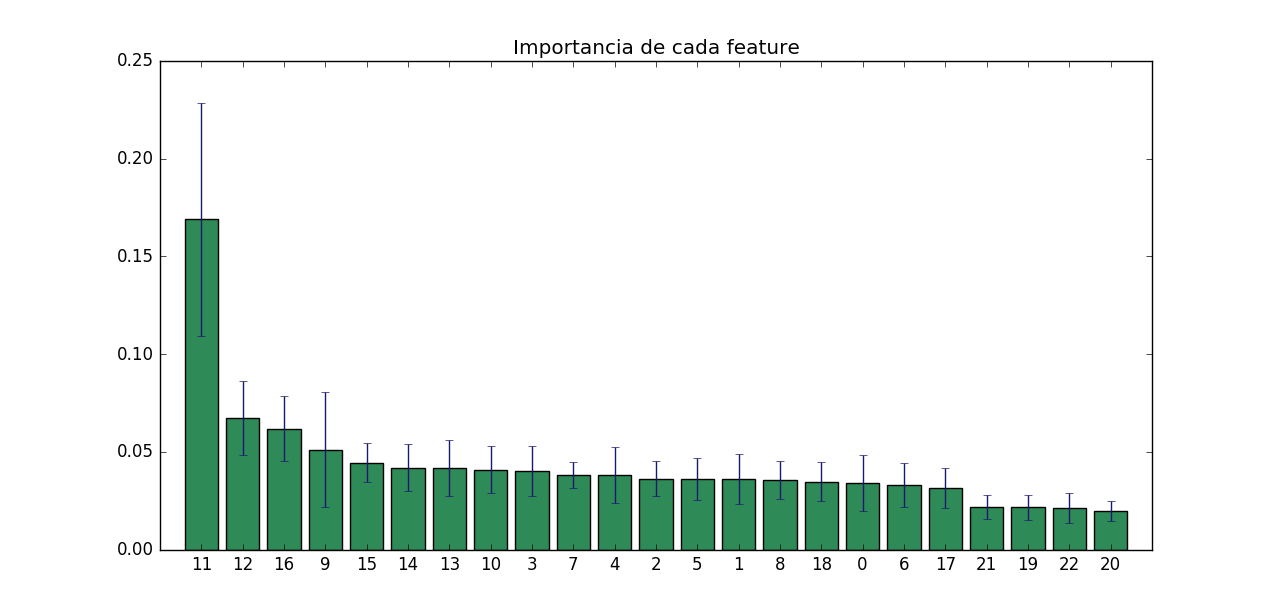
\includegraphics[width=1\textwidth]{graficos/importances.png}
  \caption{Features ordenadas según importancia}
\end{figure}

Habiendo visto estos resultados, se decidió hacer una investigación un poco más exhaustiva sobre los features más significativos, para evaluar con más exactitud qué pasa con esos rasgos en particular.

En el caso de la comparación entre pronombres femeninos y masculinos, esta medida compara la cantidades de menciones a mujeres contra la cantidad de menciones a hombres, en base a pronombres. Los nombres propios no fueron evaluados, con lo cual, una mayor cantidad de pronombres de un género se puede atribuir a una mayor cantidad de personajes de ese género o a personajes de dicho género con mayor protagonismo, y por lo tanto, con mayor número de menciones. Como se ve en el siguiente gráfico, este feature no resulta distintivo porque las mujeres escriban sólo sobre mujeres y los hombre sólo sobre hombres, sino que las curvas tienen formas totalmente diferentes: se ve una clara curva descendente entre los libros escritos por hombres que marca que la abrumadora mayoría de los autores masculinos hablan mayoritariamente sobre hombres. El promedio de los libros escritos por hombres tienen una relación de aproximadamente 0.35 de pronombres femeninos sobre pronombres masculinos. Por otro lado, en los libros escritos por mujeres se ve una variabilidad mucho mayor: en la primera figura, que sólo retrata una tasa entre 0 y 1.6, se ve poca variación, con muchos libros con personajes masculinos y otros tantos con personajes femeninos. Pero el promedio está aproximadamente en 1.1, lo que quiere decir que las menciones están casi balanceadas entre ambos géneros con un leve favorecimiento por las mujeres. Esto podría deberse a los outliers de libros que tratan exclusivamente sobre mujeres.

\begin{figure}[H]
  \centering
  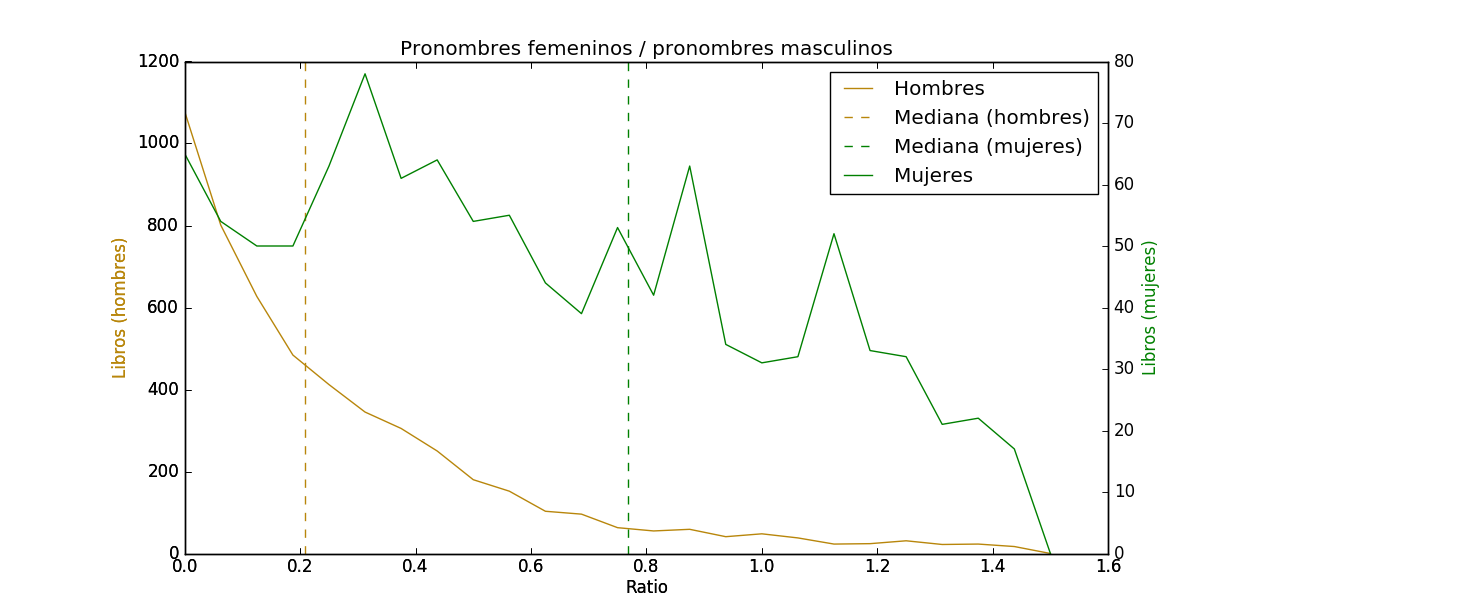
\includegraphics[width=1\textwidth]{graficos/curvas_ratio.png}
  \caption{}
\end{figure}

Si se observa la mediana en lugar del promedio, la diferencia también es muy marcada y es aún más orientada a personajes masculinos. La mitad de los libros escritos por hombres tienen una relación menor a 0.2, mientras que en los escritos por mujeres la mitad tiene apenas menos de 0.8.

\begin{figure}[H]
  \centering
  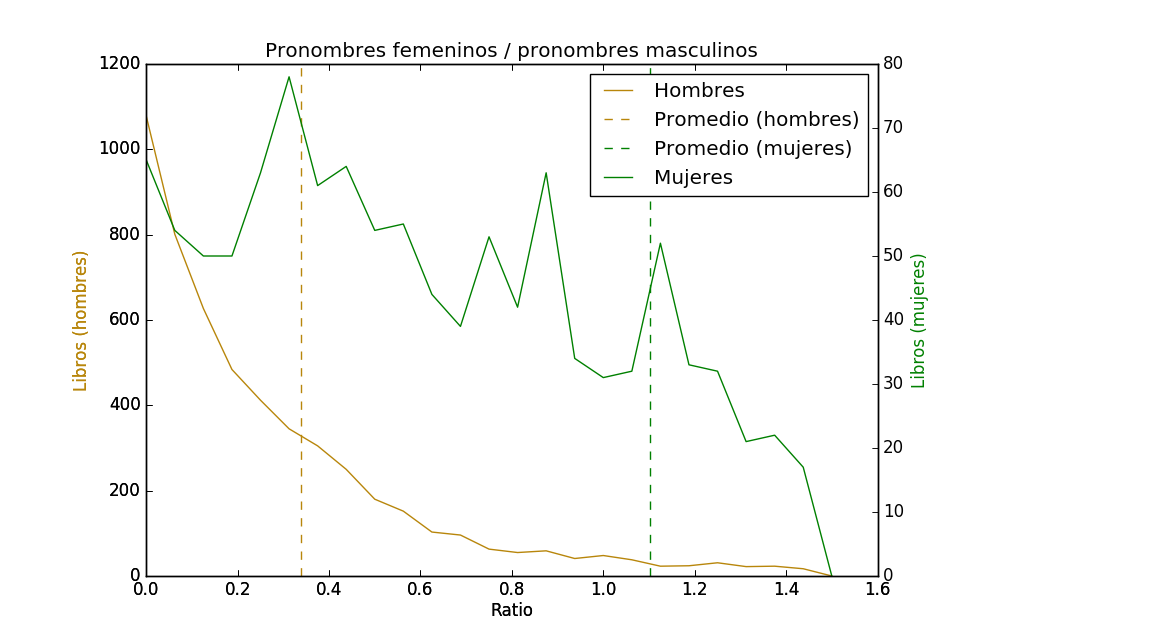
\includegraphics[width=1\textwidth]{graficos/curvas_ratio_promedio.png}
  \caption{}
\end{figure}

Las diferencias en otros features no resultaron tan marcadas, aunque sí visibles. En el caso de las menciones a niños y bebés, la mediana entre las menciones en libros escritos por mujeres y por hombres difiere notablemente, sin embargo las curvas son relativamente parecidas, con el pico de la curva de las mujeres mostrando una leve prevalencia de menciones a niños, mientras que el pico de la curva de los autores masculinos es más cercano a ninguna mención.

\begin{figure}[H]
  \centering
  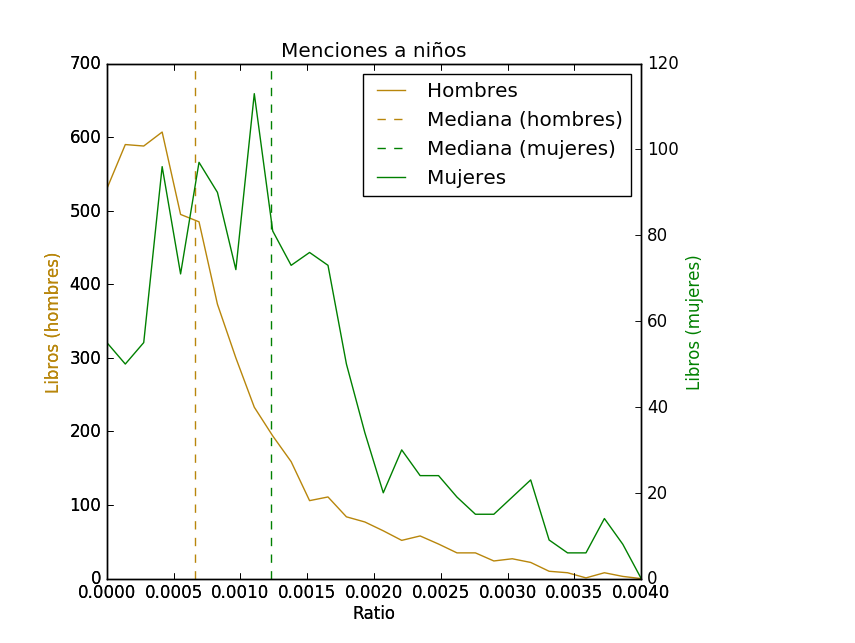
\includegraphics[width=1\textwidth]{graficos/curvas_children.png}
  \caption{}
\end{figure}

El mismo comportamiento se puede ver en menciones a colores.

\begin{figure}[H]
  \centering
  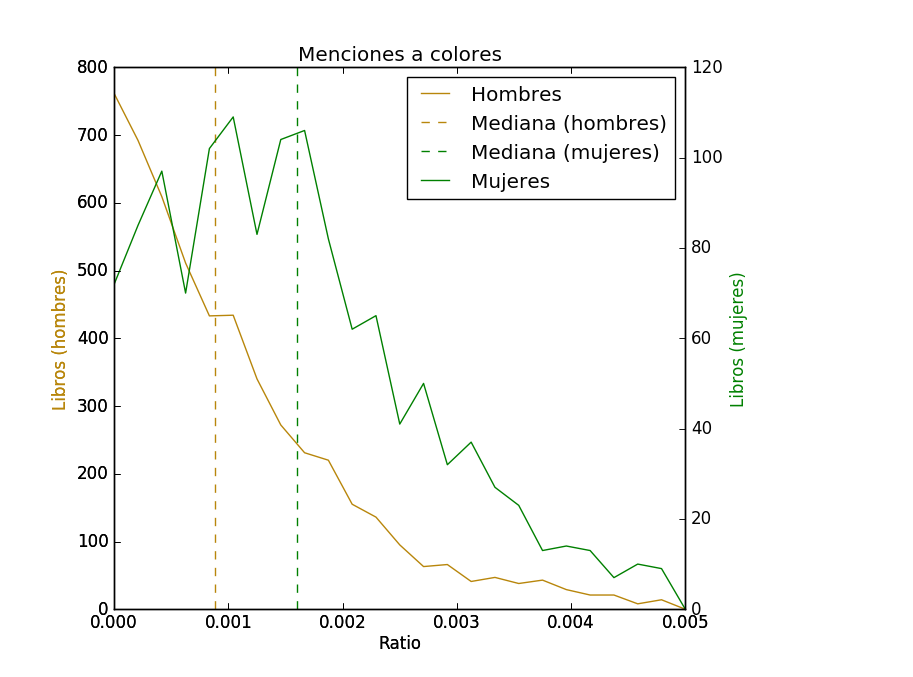
\includegraphics[width=1\textwidth]{graficos/curvas_colores.png}
  \caption{}
\end{figure}

\section{Conclusiones}

Los resultados observados no permiten vislumbrar diferencias en el estilo de escritura entre hombres y mujeres. En la bibliografía leída, y de la cual fueron obtenidos muchos de los features que se recolectaron para esta investigación, las diferencias de estilos eran de carácter más coloquial. Por ejemplo, buscar las palabras con letras repetidas pretendía encontrar escrituras especiales de algunas palabras que denotaran una emoción en particular, o que proveyeran algún efecto (como ser, “loooooove” para expresar entusiasmo en el sentimiento). Pero en una novela, este tipo de afectaciones del lenguaje no tienen lugar.

Por otro lado, al momento de buscar features que tuvieran más que ver con la temática del texto, parte de la bibliografía refería a los textos escritos por mujeres como más centrados en “sensaciones” y a los escritos por hombres como más centrados en la “acción”. En este trabajo, no se profundizó esta línea de investigación ( ya que la técnica utilizada no es la indicada para buscar cercanías por campo semántico, debido a que el análisis de porcentaje de palabras asociadas es una medida débil y que cubre pocos casos) y por ende no resultó en diferencias perceptibles. Pero la búsqueda de otra diferencia temática, como es la presencia de personajes femeninos e infantiles, sí resultó en diferencias notables.
Es evidente en los resultados que, al menos en los libros cuyos derechos de autor ya vencieron, los hombres escriben mayormente sobre personajes masculinos, o por lo pronto, que sus protagonistas son mayoritariamente hombres. Mientras que dentro de los libros escritos por mujeres hay mucha mayor variabilidad: hay libros con mayoría de referencias masculinas y otros con mayoría de referencias femeninas, pero promediando, la relación entre uno y otros es muy pareja. Si se observa la mediana, igual se puede ver que la mitad de los libros escritos por mujeres tienen mayor cantidad de referencias a personajes masculinos. Es decir, en la abrumadora mayoría de los 7000 libros analizados, la acción se centra alrededor de personajes masculinos.

\section{Discusión}

Este trabajo puede servir para aportar a una línea de investigación respecto del rol de las mujeres en la cultura, en la literatura en particular, sin embargo quedan varios análisis por hacer. En primer lugar, se podría tomar mayor cantidad de libros ampliando la selección dentro de Project Gutenberg o buscando textos de autores más contemporáneos, pero también se podría hacer un análisis más exhaustivo sobre la cantidad exacta de personajes que se reconocen por nombres en una novela, y con qué género se los identifica; investigar si dentro de aquellos escritos en primera persona se favorece a los personajes femeninos o masculinos y evaluar la preponderancia de cada personaje que aparece en el texto.

% \acknowledgement

% Sed aliquam euismod nunc nec consectetur. Fusce eget dui id tortor tristique luctus. Pellentesque elit eros, molestie et molestie vitae, laoreet in risus. Nullam ligula lectus, pulvinar eget sagittis sed, cursus ac magna. \ldots

% \suppinfo

% Ut volutpat, felis sit amet malesuada blandit, arcu sapien feugiat libero, vel interdum ipsum dolor et dolor. Fusce tortor sapien, pharetra sit amet posuere ac, viverra mollis est. Maecenas auctor ultrices quam a pharetra. Aenean ornare dictum libero vitae gravida. Mauris auctor sapien at purus accumsan lacinia.


\bibliography{sample}

\end{document}
